\section{Introduction}
Out task was to implement frequency modulation using the \textit{sine\_cordic} component we developed in the first task. The amplitude value of the input modulation signal had to be read from the ADC of the Xilinx board. Internally we generated a carrier signal with a rest frequency of 1 kHz. We altered the frequency of the carrier signal according to the amplitude of the input signal. We then wrote the altered signal to the DAC to convert the signal back to an analog wave. 


\subsection{Frequency Modulation}

Frequency modulation works by transmitting information in the form of altering a signal's frequency as pictured in figure 1. The formula we used for this purpose was: $A_csin(2\pi[f_c+f_dA_msin(f_m2\pi)])$

The variables are further explained in table 1.

\begin{figure}[H] 
\centering % centering figure 
%\scalebox{0.5} % rescale the figure by a factor of 0.8 
{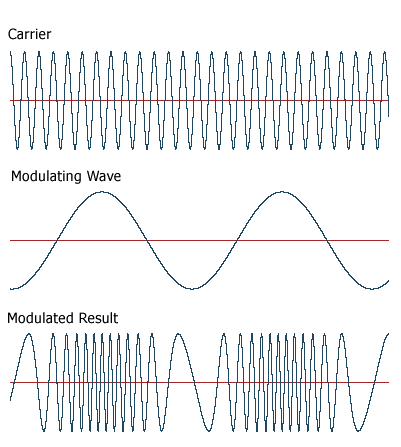
\includegraphics[height=6cm]{images/freq_mod.png}} % importing figure
\caption{Frequency modulation pictured} 
\label{fig:lorem} % labeling to refer it inside the text
\end{figure} 

\begin{table}[H] 
	\begin{center}
		\begin{tabular}{ | c | c | }
			\hline
			\textbf{Variable} & \textbf{Description} \\
			\hline
			$A_c$ & Amplitude of the carrier signal \\
			$f_c$ & Rest frequency of the carrier signal \\
			$f_d$ & Frequency deviation of the carrier signal \\
			$A_m$ & Amplitude of the modulation signal \\
			$f_m$ & Frequency of the modulation signal \\
			\hline
		\end{tabular} 
	\end{center}	
	\caption{Explanation of the variables used in the frequency modulation formula} 
\end{table} 
	


